%####PREVIO 6 IGUAL O TOMADO DE TAREA ONDA DIODO####

\documentclass{article}
\usepackage[utf8]{inputenc}
\usepackage[spanish.mexico]{babel}



\title{Dispositivos y Circuitos Electrónicos}
\author{Pablo Vivar Colina \\
Grupo 13\\
Previo práctica 6
%Tarea 14
}


\date{Marzo 2018}

\usepackage{natbib}
\usepackage{graphicx}

\begin{document}

\maketitle

\section{Rectificador de media onda}

El rectificador de media onda es un circuito empleado para eliminar la parte negativa o positiva de una señal de corriente alterna de lleno conducen cuando se polarizan inversamente. Además su voltaje es positivo.\citep{circuitoMediaOnda}

\begin{figure}[h!]
    \centering
    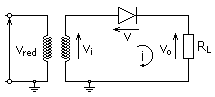
\includegraphics{Circuito_rectificador_media_onda.png}
    \caption{Caption}
    \label{fig:rectificadorMedia}
\end{figure}

\section{Rectificador de onda completa}

Un rectificador de onda completa es un circuito empleado para convertir una señal de corriente alterna de entrada (Vi) en corriente de salida (Vo) pulsante. A diferencia del rectificador de media onda, en este caso, la parte negativa de la señal se convierte en positiva o bien la parte positiva de la señal se convertirá en negativa, según se necesite una señal positiva o negativa de corriente continua.

Existen dos alternativas, bien empleando dos diodos o empleando cuatro (puente de Graetz).\citep{circuitoOnda}

\subsection{Tensión rectificada}

\begin{itemize}
    \item  Vo (corriente continua de salida) = Vi ( corriente alterna de entrada) = Vs/2 en el rectificador con diodos.
    \item  Vo = Vi = Vs en el rectificador con puente de Graetz.
\end{itemize}

   

Si consideramos la caída de tensión típica en los diodos en conducción, aproximadamente 0,7V; tendremos que para el caso del rectificador de doble onda la Vo = |Vi| - 1,4V.\citep{circuitoOnda}\\


\begin{figure}[h!]
    \centering
    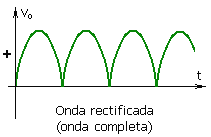
\includegraphics[scale=0.8]{OndaCompleta.png}
   % \caption{Onda Completa}
    \label{fig:my_label}
\end{figure}

\section{Puente rectificador}

El puente rectificador es un circuito electrónico usado en la conversión de corriente alterna en corriente continua. También es conocido como circuito o puente de Graetz, en referencia al físico alemán Leo Graetz (1856-1941), que popularizó este circuito inventado por el científico de origen polaco; Karol Franciszek Pollak (15 Nov. 1859 - 17 Dic.1928.)\citep{puente}



\begin{figure}[h!]
    \centering
    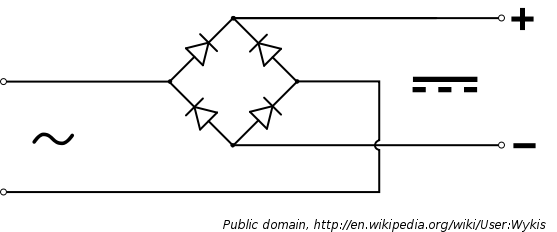
\includegraphics[scale=0.5]{PuenteDiodos.png}
    \caption{Puente de Diodos}
    \label{fig:puente de diodos}
\end{figure}

\section{Multiplicador de tensión}

Un Multiplicador de tensión es un circuito eléctrico que convierte tensión desde una fuente de corriente alterna a otra de corriente continua de mayor voltaje mediante etapas de diodos y condensadores.\citep{multiplicadorTendionWiki}

\begin{figure}[h!]
    \centering
    \includegraphics[scale=0.5]{Imagenes/Vmult.png}
    \caption{Multiplicador de voltaje}
    \label{fig:multV1}
\end{figure}

\subsection{Funcionamiento}

Un multiplicador de tensión sin cargar con una impedancia se comporta como un condensador, pudiendo proporcionar transitorios de elevada corriente, lo que los hace peligrosos cuando son de alta tensión. Habitualmente se agrega una resistencia en serie con la salida para limitar este transitorio a valores seguros, tanto para el propio circuito como ante accidentes eventuales.\citep{multiplicadorTendionWiki}

\begin{figure}[h!]
    \centering
    \includegraphics[scale=0.10]{Imagenes/voltageMult.png}
    \caption{Multiplicador de voltaje}
    \label{fig:multV2}
\end{figure}

\subsection{Voltaje de Ruptura}

Mientras esta configuración puede ser utilizada para generar miles de voltios a la salida, los componentes de las etapas individuales no requieren soportar toda la tensión sino solo el voltaje entre sus terminales, esto permite aumentar la cantidad de etapas según sea necesario sin aumentar los requerimientos individuales de los componentes.Lo cual es una gran ventaja en la producción de este tipo de circuitos que son de un muy gran provecho.\citep{multiplicadorTendionWiki}

\section{Filtro para la corriente alterna rectificada}

La onda rectificada se pasa por un filtro, el cual está constituido por uno o mas condensadores electrolíticos, para obtener un nivel de tensión continua mucho mejor que el que se obtiene con solo la rectificación con el puente de diodos, en la imagen siguiente se representa como estaría el circuito para la fuente de alimentación hasta el momento con el condensador de filtro incluido.\citep{FiltroParaCorrienteAlterna}

\begin{figure}[h!]
    \centering
    \includegraphics[scale=0.16]{Imagenes/Condensador-filtro.jpg}
    \caption{Puente de diodos}
    \label{fig:puentDiod1}
\end{figure}

El voltaje de salida rectificado tiene un valor de voltaje en continua igual a Vcd = 2(Vp-1,4)/π también se ha visto que la frecuencia del voltaje rectificado es el doble de la frecuencia del voltaje que sale del secundario del transformador, por ejemplo si la frecuencia de voltaje sin rectificar es de 50Hz(eso depende del país), entonces la frecuencia del voltaje rectificado será 100Hz;con el condensador de filtro lo que logra es mejorar el nivel de salida en continua, el cual se aproximará  al valor de (Vp-1,4) como se aprecia en la figura \ref{fig:rizado}.\\

\begin{figure}[h!]
    \centering
    \includegraphics[scale=0.5]{Imagenes/rizov.jpg}
    \caption{Gráficas de rizado}
    \label{fig:rizado}
\end{figure}

 Para el primer ciclo del voltaje rectificado, que sale  del puente de diodos, que luego pasa por el filtro (el condensador electrolítico), ocurre lo siguiente, en un inicio el voltaje del ciclo aumenta desde 0V hasta (Vp-1,4)V  el condensador se cargará a través de los diodos que estén activos (D1 y D2 o D3 y D4) hasta (Vp-1,4)V, donde Vp es el voltaje pico de la tensión alterna rectificada, luego el voltaje en el ciclo empezará a disminuir, esto provocará que los diodos que estaban conduciendo se polaricen en inversa y dejen de conducir o se apaguen, ya que la tensión del ánodo de los diodos que es la tensión que sale del secundario del transformador se hará menor que la tensión del cátodo de los diodos que es el valor al cual se ha cargado el condensador, esto porque la constante de tiempo de descarga del condensador es mucho mayor que el periodo de la tensión rectificada, en ese momento el condensador empezará a descargar a través de la resistencia de carga, pero esa descarga será mucha mas lenta que la carga que es a través de los diodos, como el periodo del ciclo es menor que el tiempo de descarga del condensador, llegará un momento mientras el condensador está descargando que la tensión del siguiente ciclo se haga mayor a la tensión que tiene el condensador y provoque que el otro par de diodos diodos se activen y se polaricen en directa y conduzcan la corriente, esto provocará que el condensador vuelva a cargarse hasta (Vp-1,4)V; luego el ciclo disminuirá su valor. los diodos que conducían se apagarán y el condensador descargará, en el siguiente ciclo el otro par de diodos se activarán el condensador nuevamente se cargará y todo ese proceso se repetirá para los siguientes ciclos del voltaje rectificado: ese proceso se puede ver en el esquema anterior en color rojo, se puede ver que solo en el primer ciclo el condensador cargará de 0V a (Vp-1,4)V, luego el condensador empezará a descargar y cargar como se observa en la figura. La forma de onda en color rojo será la que llegue al  filtro de la tensión rectificada en color azul.\citep{FiltroParaCorrienteAlterna}\\

A la forma de onda obtenida en la figura en color rojo se le llama rizado si ahora se mide con un multitester la tensión continua sobre la resistencia de carga se observará que esa medida se aproxima a (Vp-1,4), pero aún no es totalmente continua, la diferencia entre el valor máximo y mínimo del rizado se denomina tensión de rizado pico a pico Vppr y tiene un valor que se puede aproximar con la siguiente fórmula:\citep{FiltroParaCorrienteAlterna}\\

\begin{equation}
    V_{ppr}=\frac{I}{fC}
\end{equation}

Donde I es la corriente continua que se quiere que suministre la fuente de alimentación, f es la frecuencia del rizado que será igual a la frecuencia de la tensión rectificada, que es el doble de la frecuencia del la tensión obtenida en el secundario del transformador que es 50Hz o 60Hz(eso depende del país), por ejemplo si la frecuencia es 50Hz, entonces la frecuencia de rizado será 100Hz; y C es la capacitancia del condensador utilizado como filtro; para que la tensión medida sea totalmente continua, será necesario hacer el rizado lo menor posible esto es  Vppr lo mas pequeño posible.\citep{FiltroParaCorrienteAlterna}\\

Para hacer el Vppr pequeño se tendría que disminuir la corriente, pero en la fuente de alimentación se quiere que este sea lo mayor posible ya que si se disminuye la corriente la fuente no servirá de mucho, otra opción sería aumentar la frecuencia de rizado, pero la frecuencia es una constante 100Hz o 120Hz; otr< opción que queda es que la capacitancia del condensador de filtro sea un valor grande, lo  cual puede ser, pero resulta que la capacitancia no debe tener un valor demasiado grande ya que esto afectaría a los diodos y a la bobina del del secundario del transformador.\citep{FiltroParaCorrienteAlterna}



\bibliographystyle{plain}
\bibliography{Referencias.bib}


\end{document}